\documentclass[a4paper,11pt]{article}
% Compile with XeLaTeX or LuaLaTeX (arXiv auto-detects via fontspec).
% Japanese glyphs use Harano Aji, which ships with TeX Live (and arXiv).
\usepackage{iftex}
\ifPDFTeX
  \usepackage[utf8]{inputenc}
  \usepackage[T1]{fontenc}
\else
  \usepackage{fontspec}
  \usepackage{xeCJK}
  \setCJKmainfont{HaranoAjiMincho-Regular.otf}
\fi
\usepackage{amsmath, amssymb, amsthm}
\usepackage{graphicx}
\usepackage{hyperref}
\usepackage{geometry}
\geometry{margin=1in}
\usepackage{cite}

% Untranslated concept term (Japanese): Jōcho (情緒)
\newcommand{\jocho}{\emph{J\={o}cho}}

\title{\textbf{Spirit in Physics:}\\
\large constructing the self as an information-geometric (tensor) space\\
from word association and physiology}
\author{
    Jun Kawasaki$^{1}$, Kazuki Tainaka$^{2}$, Tomonori Takeuchi$^{3}$ \\
    \small $^{1}$Graduate School of Medical and Dental Sciences, Niigata University \\
    \small $^{2}$Brain Research Institute, Niigata University, Japan \\
    \small $^{3}$Department of Biomedicine, Aarhus University, Denmark \\
    \small \texttt{root@junkawasaki.com}
}
\date{June 28, 2026}

\begin{document}
\maketitle

\begin{abstract}
We take one assumption seriously and build on it: the conscious self---``spirit''---\emph{is} information. If information is physical (Shannon--Jaynes--Landauer), then a self made of information is a physical object, and the right way to study it is not to test a correlation but to \textbf{construct} it. We therefore give a \textbf{constructive} operational definition: the spirit of an individual \emph{is} the information-geometric space we build from that person's own signals---word associations (Jung), reaction times, and physiological response---in which charged clusters (Jungian \emph{complexes}) and their boundaries with concepts become geometric structure. The boundary of the self is, in principle, fixed physiologically by a rubber-hand-illusion paradigm; the conceptual structure is laid down by the word-association method. We render each individual as a third-order tensor (word $\times$ session $\times$ bodily-feature), embed it spectrally into a per-person ``spirit space,'' and read complexes off as high-energy regions. \textbf{Information $=$ physics $=$ this mathematical space}: the model is not a description of the spirit, it is taken to be the spirit. In a pilot ($N=5$ analyzed of 11; responses transcribed automatically) we build individual spirit spaces, locate their complexes, and use a tensor decomposition to look for a shared component---a candidate \emph{collective unconscious}. It is faint but above chance (inter-subject $r=+0.07$, $p=0.04$); its variance share is not estimable at $N=5$ (the apparent $\sim$25\% sits at the mechanical null). The spirit space is, at this scale, overwhelmingly individual. We present this as a reproducible construction and visualization (the full pipeline runs as a checkpointed StateGraph), not as a confirmatory study; the physiological boundary (RHI) data are the next installment.
\end{abstract}

\section{Introduction}
The concept of ``spirit'' has stayed outside empirical science for want of a physically grounded, measurable definition. Rather than ask whether spirit \emph{can} be reduced to physics, we adopt a constructive stance: \textbf{assume} the self is information, build the object that assumption implies, and see what it looks like. If the assumption is wrong the construction will be empty or structureless; if it is right, an individual's spirit should appear as concrete geometry recoverable from that individual's own signals.

We keep the Japanese term \jocho{} (情緒) untranslated for the layer of lived, meaning-laden experience not captured by ``emotion'' or ``affect,'' following Kiyoshi Oka \cite{Oka1963,Oka2008}. Our contribution is constructive and infrastructural, not a hypothesis test: (i) an operational identity---\emph{the spirit of a person is the information-geometric space built from their associations and physiology}; (ii) a concrete construction of that space (tensor $\to$ spectral embedding) in which Jungian complexes are high-energy regions; and (iii) a decomposition that separates the individual space from a shared, collective component. The analytical-psychology vocabulary (Section~\ref{sec:interp}) is an interpretive layer over the constructed geometry.

\section{Theoretical Framework}
We make three assumptions that turn ``spirit'' into a constructible physical object.

\subsection{Assumption 1: Information is physical}
\textbf{Shannon (1948)} defined information entropy $H$ \cite{Shannon1948}; \textbf{Jaynes (1957)} showed it is formally the thermodynamic entropy $S$ \cite{Jaynes1957}; \textbf{Landauer (1961)} showed information processing has an energetic cost $k_B T\ln 2$ \cite{Landauer1961}, experimentally verified \cite{Berut2012}. We use this chain as the \emph{motivating} grounding for treating an informational self as physical; we do not measure $k_BT$ or entropy production here.

\subsection{Assumption 2: The self (spirit) is information}
The \textbf{rubber-hand illusion} \cite{Botvinick1998} shows the self-boundary is a malleable informational construct with a physiological signature---so the boundary of the self can, in principle, be \emph{measured} (as a bodily response) rather than assumed. \textbf{Jung's word association} \cite{Jung1910} shows the psyche is organized into \emph{complexes}: clusters of charged concepts with measurable reaction times and autonomic responses. Together they license representing a self as charged structure in an informational space.

\subsection{Assumption 3: Spirit as an open informational system}
A self persists by exchanging information and entropy with its environment \cite{Schrodinger1944}; the \textbf{free-energy principle} \cite{Friston2010} casts this as surprisal minimization. We adopt the resulting picture---a self is a structured region of an informational state space---and take the constructive step the principle invites: \emph{build} that state space from data. Non-equilibrium thermodynamics \cite{Seifert2012,Parrondo2015} and feedback control \cite{SagawaUeda2010} motivate, but are not invoked quantitatively in, the present pilot.

\section{Structural Interpretation}\label{sec:interp}
We interpret the constructed geometry with analytical psychology:
\begin{itemize}
    \item \textbf{Complex:} an energy-charged region of the individual's space (short or labile reaction time, elevated autonomic response).
    \item \textbf{Archetype:} a structural template recurring \emph{across} individuals---hence a property of the shared component (Section~\ref{sec:tensor}).
    \item \textbf{Shadow:} suppressed, less reproducible parts of a complex.
\end{itemize}

\section{Constructing the individual spirit space}\label{sec:method}
We instantiate the spirit of a person as follows. Each stimulus word is presented (Jung's method); the spoken association is transcribed automatically (we reconstruct $851$ stimulus$\to$response pairs across the pilot from the recordings), and two bodily readouts are taken per trial: \textbf{response latency} (a temporal index of processing) and \textbf{skin potential} $\Delta SP$ (electrodermal response). The rubber-hand-illusion paradigm provides the bodily \emph{boundary} of the self under congruent versus incongruent stimulation; those data are pending and the present construction uses the word-association and physiological channels.

For one individual, let each node $w$ (a stimulus and/or its response concept) carry a bodily feature vector $x_w$ (standardized latency and skin potential, per session). We define the \textbf{charge / energy} of a node intrinsically,
\begin{equation}
    E(w) \;=\; z\big(\text{latency}(w)\big) + z\big(\Delta SP(w)\big),
    \label{eq:energy}
\end{equation}
build a similarity kernel between nodes, $W_{ij}=\exp(-\lVert x_i-x_j\rVert^2/\sigma^2)$ with $\sigma$ the median pairwise distance, and embed the nodes by the low-lying eigenvectors of the symmetric normalized graph Laplacian $L_{\mathrm{sym}}=I-D^{-1/2}WD^{-1/2}$. \textbf{This embedded, energy-weighted geometry is the spirit space of the individual.} We use two related notions of energy, and keep them distinct: the intrinsic \emph{node charge} $E(w)$ of Eq.~\eqref{eq:energy} (latency$+$arousal; this colours the charge geometry of Figs.~\ref{fig:landscape}--\ref{fig:individual}), and the \emph{manifold energy} of a node---its radius from the centroid of the spectral embedding---which is what ranks nodes into complexes; the two covary (within-individual $r\approx0.52$ between node charge and manifold energy; both rise with latency and arousal). A \emph{complex} is a high-energy region, and its boundary with neutral concepts is where the energy falls off. The construction is intrinsic---no cross-person normalization, no notion of how ``common'' a response is, enters it. We take this constructed object to be the spirit: information $=$ physics $=$ this space.

\paragraph{Well-posedness (a stipulative identity, not a tested hypothesis).} To forestall a category error we state the logic explicitly. (i) ``The spirit of a person \emph{is} this space'' is a \textbf{stipulative operational definition}, not an empirical claim to be confirmed by a $p$-value. (ii) What is empirically at stake is whether the construction is \emph{non-empty}: a structureless result would show a flat Laplacian spectrum (no spectral gap), node energy uncorrelated with node identity, and no reproducible high-energy regions. (iii) We instead find structure on all three counts (Sections~\ref{sec:pilot}--\ref{sec:tensor}: spectral gap $\approx0.19$, participation ratio $\approx10.9$, low-rank Tucker geometry, reproducible complexes), so the construction is non-empty---the definition picks out something real, whose \emph{scientific} content (individual structure, shared component) is then measured with appropriate restraint.

\section{Pilot: individual spirit spaces and their complexes}\label{sec:pilot}
We recruited 11 participants and analyze the $N=5$ with synchronized, clock-aligned continuous skin potential. Across these, $970$ trials were recorded; $945$ have a valid skin-potential response window (used for the charge geometry) and $851$ also carry a transcribed verbal response (used to label nodes). Each individual completed two test--retest sessions of an identical $\sim$100-word list. For each we build the spirit space of Section~\ref{sec:method} and read off its energy geometry.

\begin{figure}[t]
    \centering
    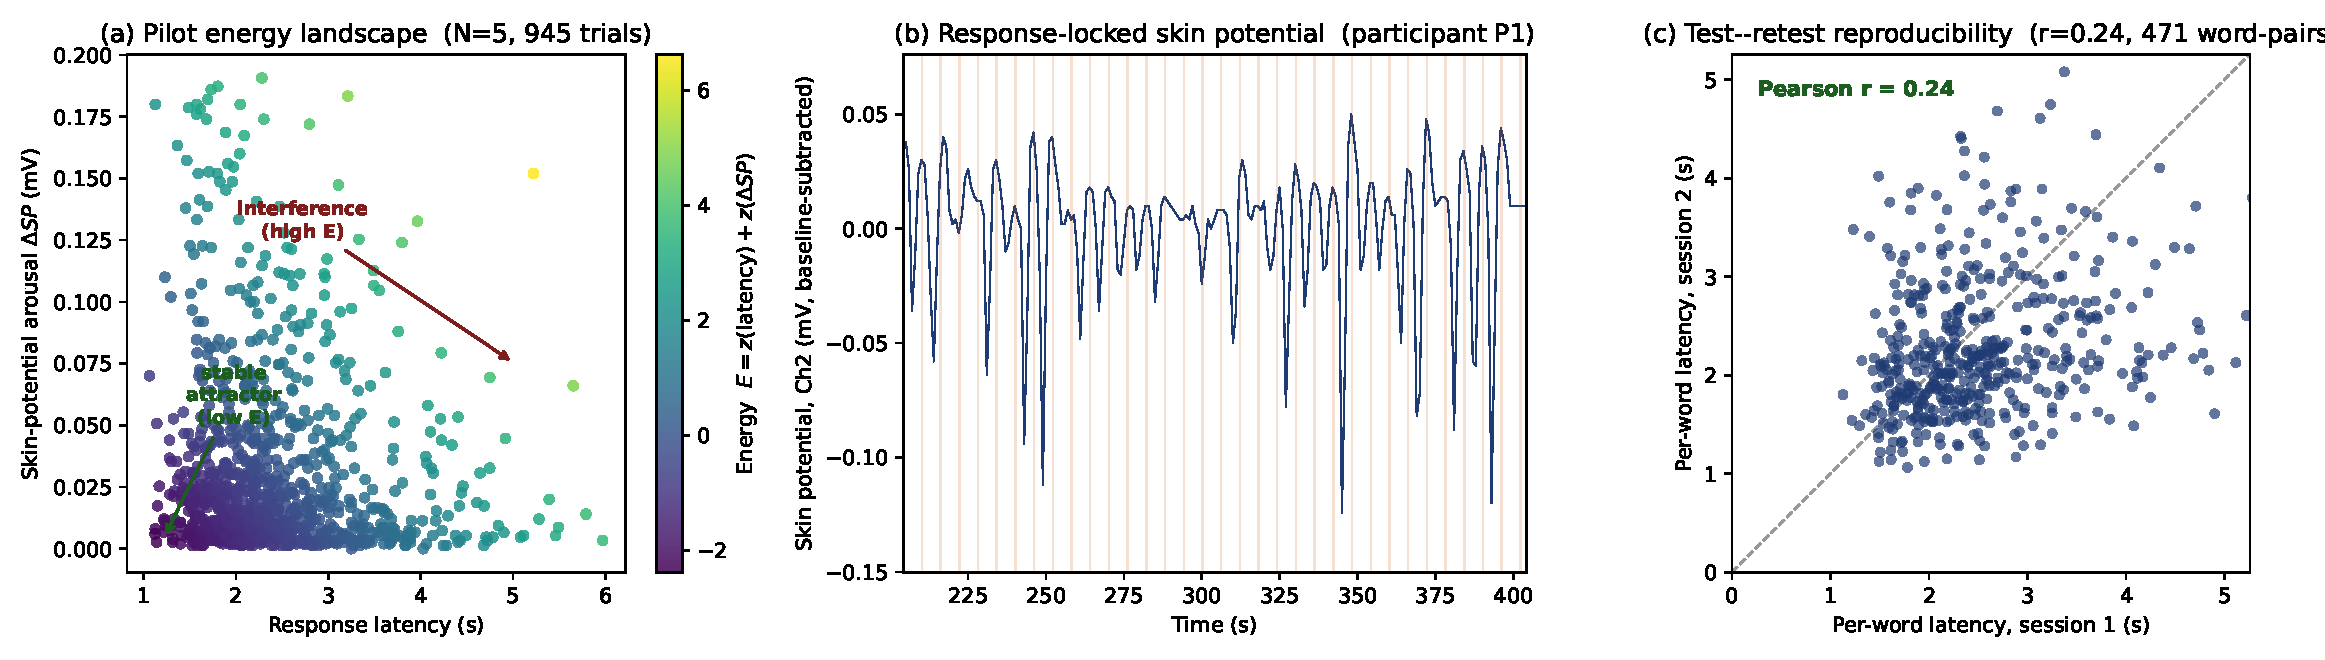
\includegraphics[width=\textwidth]{fig_landscape.pdf}
    \caption{\textbf{The constructed spirit space (energy geometry).}
    (a) Every node is a word-association trial placed by response latency and
    skin-potential charge $\Delta SP$ and coloured by node energy $E$
    (Eq.~\eqref{eq:energy}); low-$E$ \emph{attractor} regions (neutral concepts)
    and high-$E$ \emph{complex/interference} regions emerge intrinsically, with
    no popularity or frequency normalization. (b) Skin potential for one
    individual; vertical lines mark word onsets---the physiological signal from
    which the boundary is read. (c) Stability of the space across the two
    sessions (per-word latency, identical list; $r=0.24$). Generated by
    \texttt{scripts/make\_landscape\_figure.py}.}
    \label{fig:landscape}
\end{figure}

\paragraph{Complexes as high-energy regions.} The energy geometry separates two intrinsic regimes (Fig.~\ref{fig:landscape}a): low-$E$ attractor regions (fast, low-arousal, reproducible nodes---neutral concepts) and high-$E$ regions (slow and/or high-arousal, less reproducible nodes), which are the candidate \emph{complexes}. For the pilot cohort the high-energy region is populated by items such as \textit{door}~(ドア), \textit{big}~(大きい), \textit{wash}~(洗う), \textit{habit}~(癖), \textit{expensive}~(高価な), and the low-energy attractor by concrete neutral items---\textit{ink}~(インク), \textit{tree}~(木), \textit{book}~(本), \textit{finger}~(指), \textit{dance}~(踊る). These charged regions are exactly what Jung's complex predicts as measurable structure; here they are read directly from the body. Figure~\ref{fig:individual} shows the five individual spirit spaces---each a spectral geometry of that person's own nodes, coloured by energy---making concrete the claim that the constructed space \emph{is} the individual's spirit. We quantify how individual they are by orthogonal-Procrustes disparity: between-person disparity ($1.74$) exceeds the within-person, session-to-session disparity ($1.61$) only marginally (ratio $1.08$, bootstrap $95\%$ CI $[0.46,\,1.08]$---not reliably above $1$). So although the panels look distinct, individual separation is \emph{not statistically established} at $N=5$; it is a target for the powered study, stated here without overclaim.

\begin{figure}[t]
    \centering
    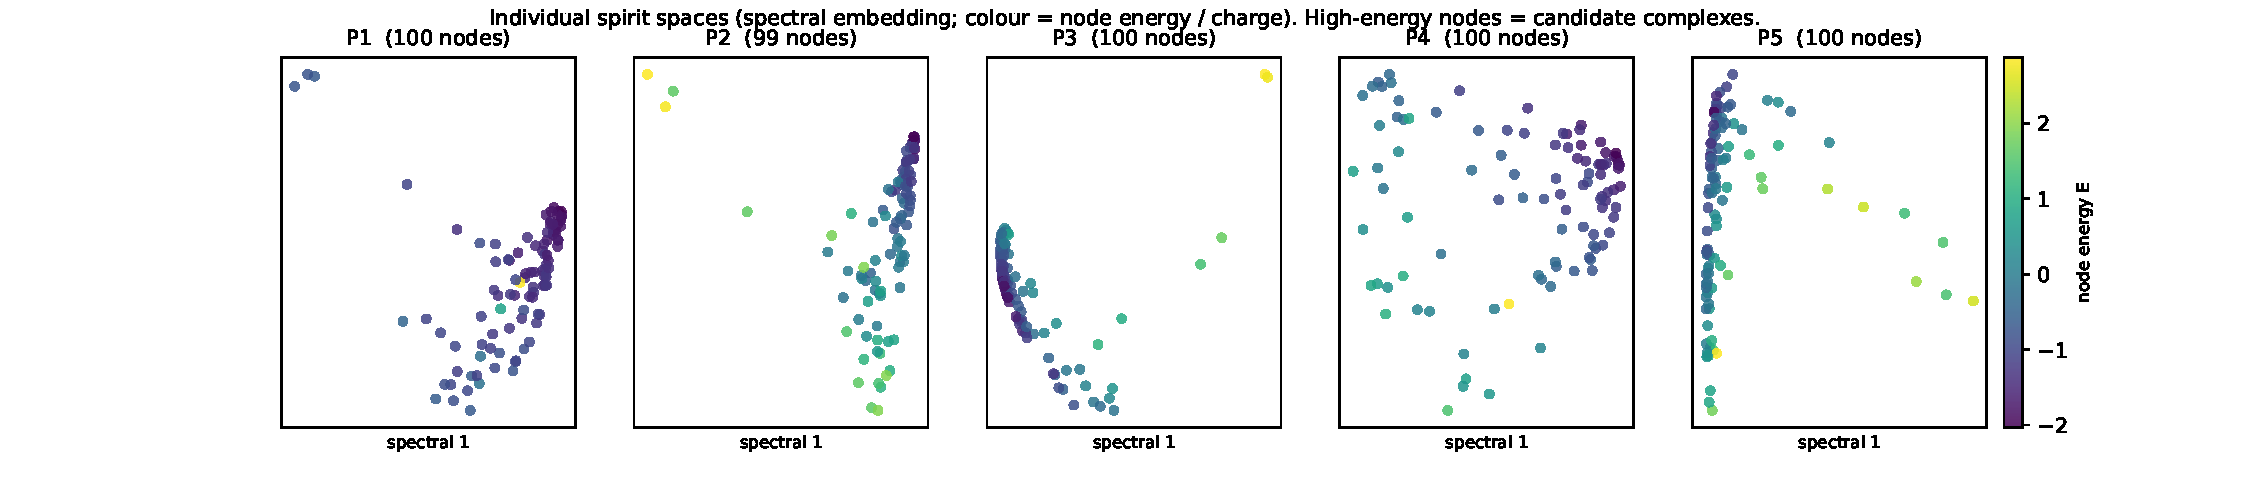
\includegraphics[width=\textwidth]{fig_individual_spirit.pdf}
    \caption{\textbf{Individual spirit spaces.} Each panel is one participant's
    own constructed space (spectral embedding of their word nodes from latency
    and skin potential), coloured by node energy $E$ (Eq.~\eqref{eq:energy}).
    The geometries are visibly distinct across individuals; high-energy (bright)
    nodes are that person's candidate complexes. Generated by
    \texttt{scripts/plot\_individual\_spirit.py}.}
    \label{fig:individual}
\end{figure}

\paragraph{The space is dynamic and individual.} Re-exposure (session 1 $\to$ 2) reshapes the space: response latency falls in $3/5$ individuals (mean $-0.25$\,s) and skin-potential charge in $4/5$ (mean $-0.004$\,mV), i.e.\ the geometry relaxes as concepts become familiar. The space is also strongly \emph{individual}: per-word charge is only weakly shared across people (next section).

\section{Individual vs.\ collective: tensor decomposition}\label{sec:tensor}
To separate what is idiosyncratic to a person from what is shared, we stack the cohort as a third-order tensor $\mathcal{T}\in\mathbb{R}^{P\times W\times F}$ ($P=5$ individuals, $W=99$ shared words, $F=3$ bodily features) and analyze its geometry; the full pipeline (build $\to$ tensorize $\to$ spectral $\to$ Tucker $\to$ summarize) runs as a checkpointed \texttt{langgraph-clj} StateGraph.

\paragraph{Shape of the shared space.} A graph-Laplacian spectral embedding of the words (Fig.~\ref{fig:manifold}a,b) shows a \textbf{spectral gap} $\approx0.19$ and a participation ratio of $\approx10.9$ effective modes: the shared spirit space is genuinely multi-dimensional yet has a dominant collective coordinate. A Tucker (HOSVD) decomposition at ranks $[3,6,3]$ reconstructs $76\%$ of the variance and saturates near $0.83$ by word-mode rank $\approx12$ (Fig.~\ref{fig:manifold}c). Crucially the decomposition factorizes the tensor into a \textbf{participant mode (the individual spirit)} and \textbf{shared word-modes (structure common across people)}.

\paragraph{The collective component (a candidate collective unconscious).} How much of the geometry is shared? We are deliberately conservative here, because with only $P=5$ rows the first principal component mechanically absorbs a large share. Against a within-subject shuffle null: the inter-subject per-word charge correlation is weak but \emph{above chance} ($\bar r=+0.065$, permutation $p=0.038$), whereas the first-PC share ($27\%$) is \emph{indistinguishable} from its mechanical null ($\approx26\%$, $p=0.21$)---so the $27\%$ is \textbf{not} evidence of shared structure, only the baseline. The honest reading is therefore narrow: there is a faint, above-chance shared component (the candidate \emph{collective unconscious}), but its magnitude cannot be estimated at $N=5$, and the variance-share figure should not be read as ``$25\%$ collective.'' This shared component is the natural place to look for cultural/population structure (comparing tensor spaces across language or culture) in the powered study (Fig.~\ref{fig:collective}).

\begin{figure}[t]
    \centering
    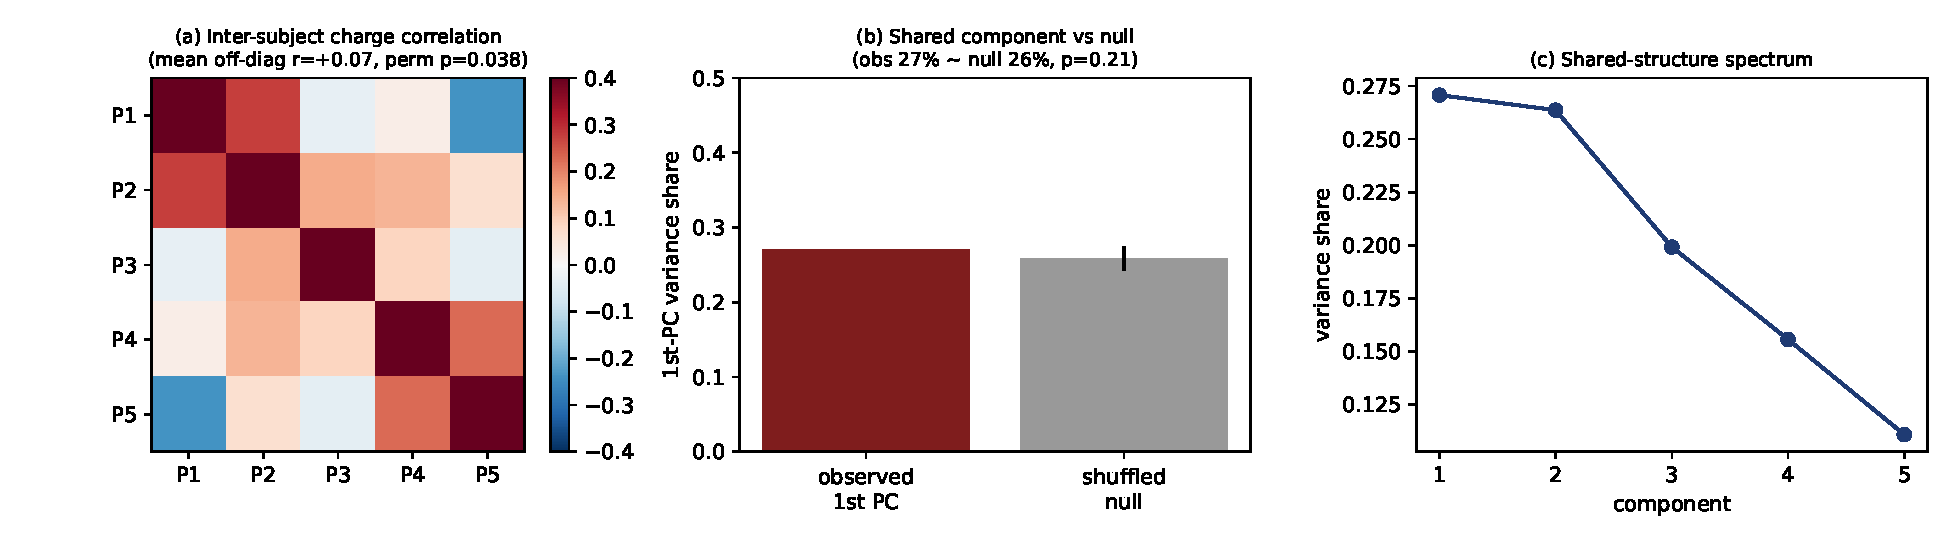
\includegraphics[width=\textwidth]{fig_collective.pdf}
    \caption{\textbf{Individual vs.\ collective structure.}
    (a) Inter-subject correlation of per-word charge (mean off-diagonal
    $r=+0.07$, permutation $p=0.038$): a faint but above-chance shared signal on
    a largely private space. (b) The first-PC variance share ($27\%$) sits at
    its shuffle-null baseline ($\approx26\%$, $p=0.21$)---i.e.\ a mechanical
    artifact of $P=5$, \emph{not} evidence of a large collective component.
    (c) The shared-structure spectrum. Generated by
    \texttt{scripts/plot\_individual\_spirit.py}.}
    \label{fig:collective}
\end{figure}

\begin{figure}[t]
    \centering
    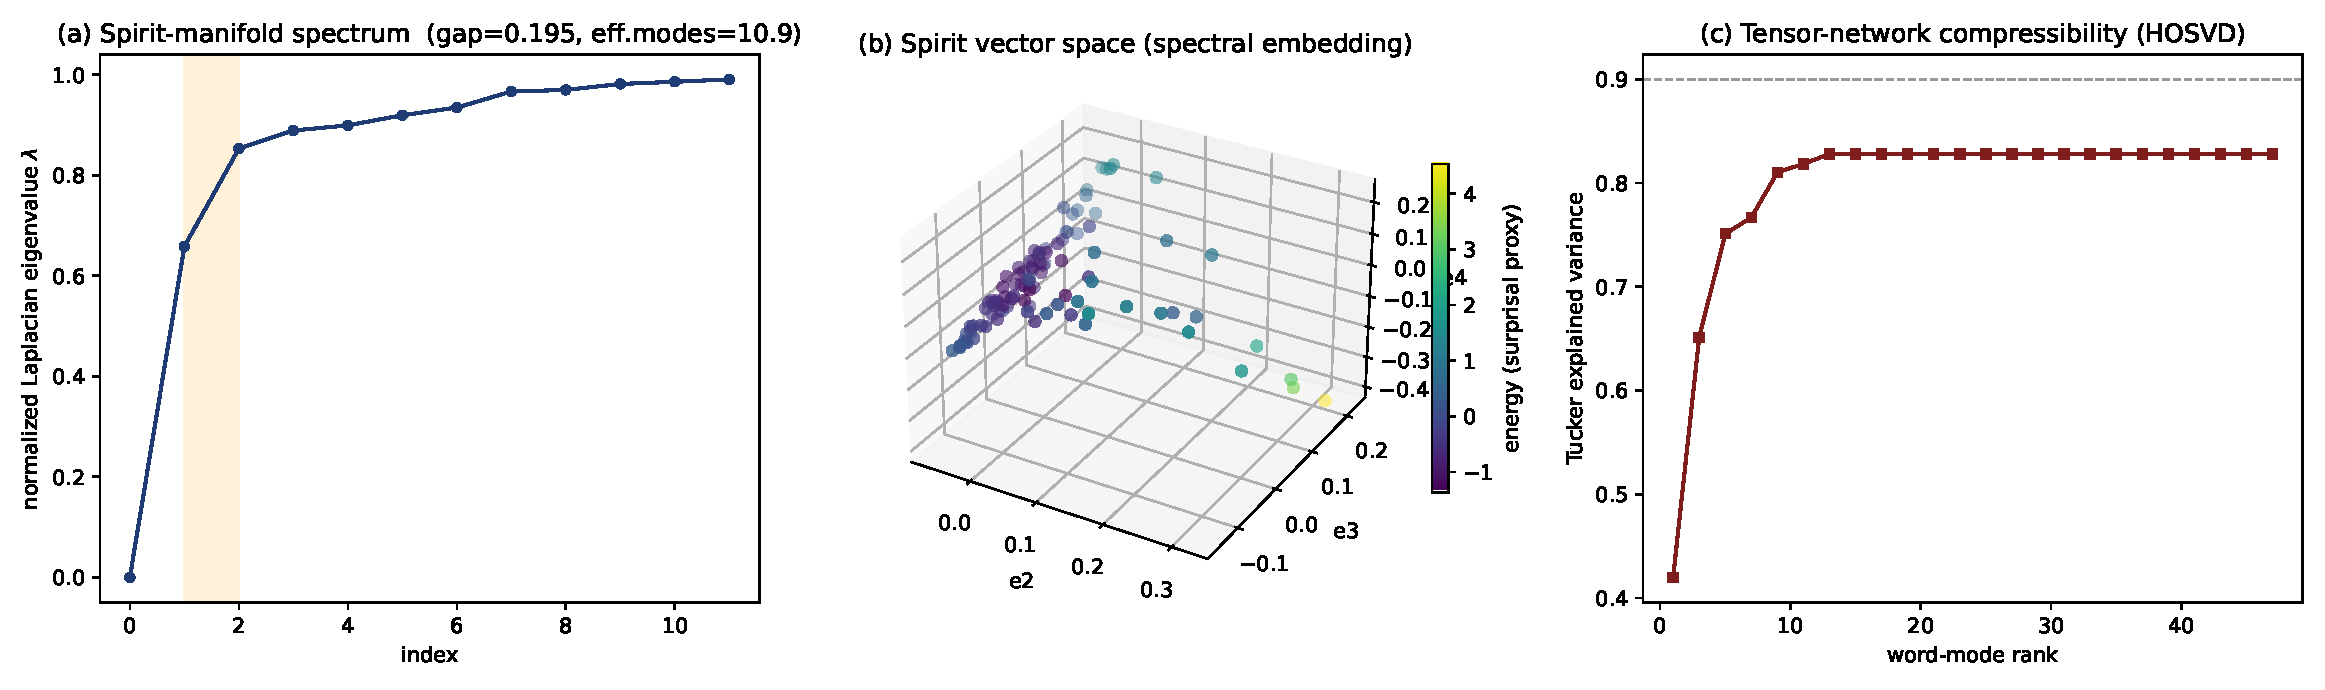
\includegraphics[width=\textwidth]{fig_spirit_manifold.pdf}
    \caption{\textbf{The spirit space as geometry: individual and shared structure.}
    (a) Normalized graph-Laplacian spectrum; the gap ($\approx0.19$) marks the
    dominant collective coordinate (effective modes $\approx10.9$).
    (b) Three-dimensional spectral embedding---the shared \emph{spirit vector
    space}---with words coloured by energy.
    (c) Tucker (HOSVD) explained variance vs.\ word-mode rank; the tensor is
    low-rank ($\approx0.83$ by rank $\approx12$) with an irreducible individual
    residual. These are descriptive geometry over $P=5$, not inferential
    population statistics. Computed by the \texttt{langgraph-clj} StateGraph over
    \texttt{scripts/spirit\_tensor.py}.}
    \label{fig:manifold}
\end{figure}

\paragraph{Visualization.} Because the construction \emph{is} the spirit, it is also something one can look at. Figure~\ref{fig:awe} renders the same quantities---spectral-embedding positions, node energy, and the affinity kernel---through the auxiliary physical pictures of Section~\ref{sec:interp}: the energy landscape as a heat-kernel field (curved-manifold gravity wells), the kernel as luminous filaments, and complexes as bright bioluminescent concentrations, with each individual a distinct nebula beneath the shared manifold. The rendering is generated from the same pipeline (\texttt{scripts/render\_spirit\_awe.py}); it adds no data, only a faithful, high-altitude view of the constructed object.

\begin{figure}[t]
    \centering
    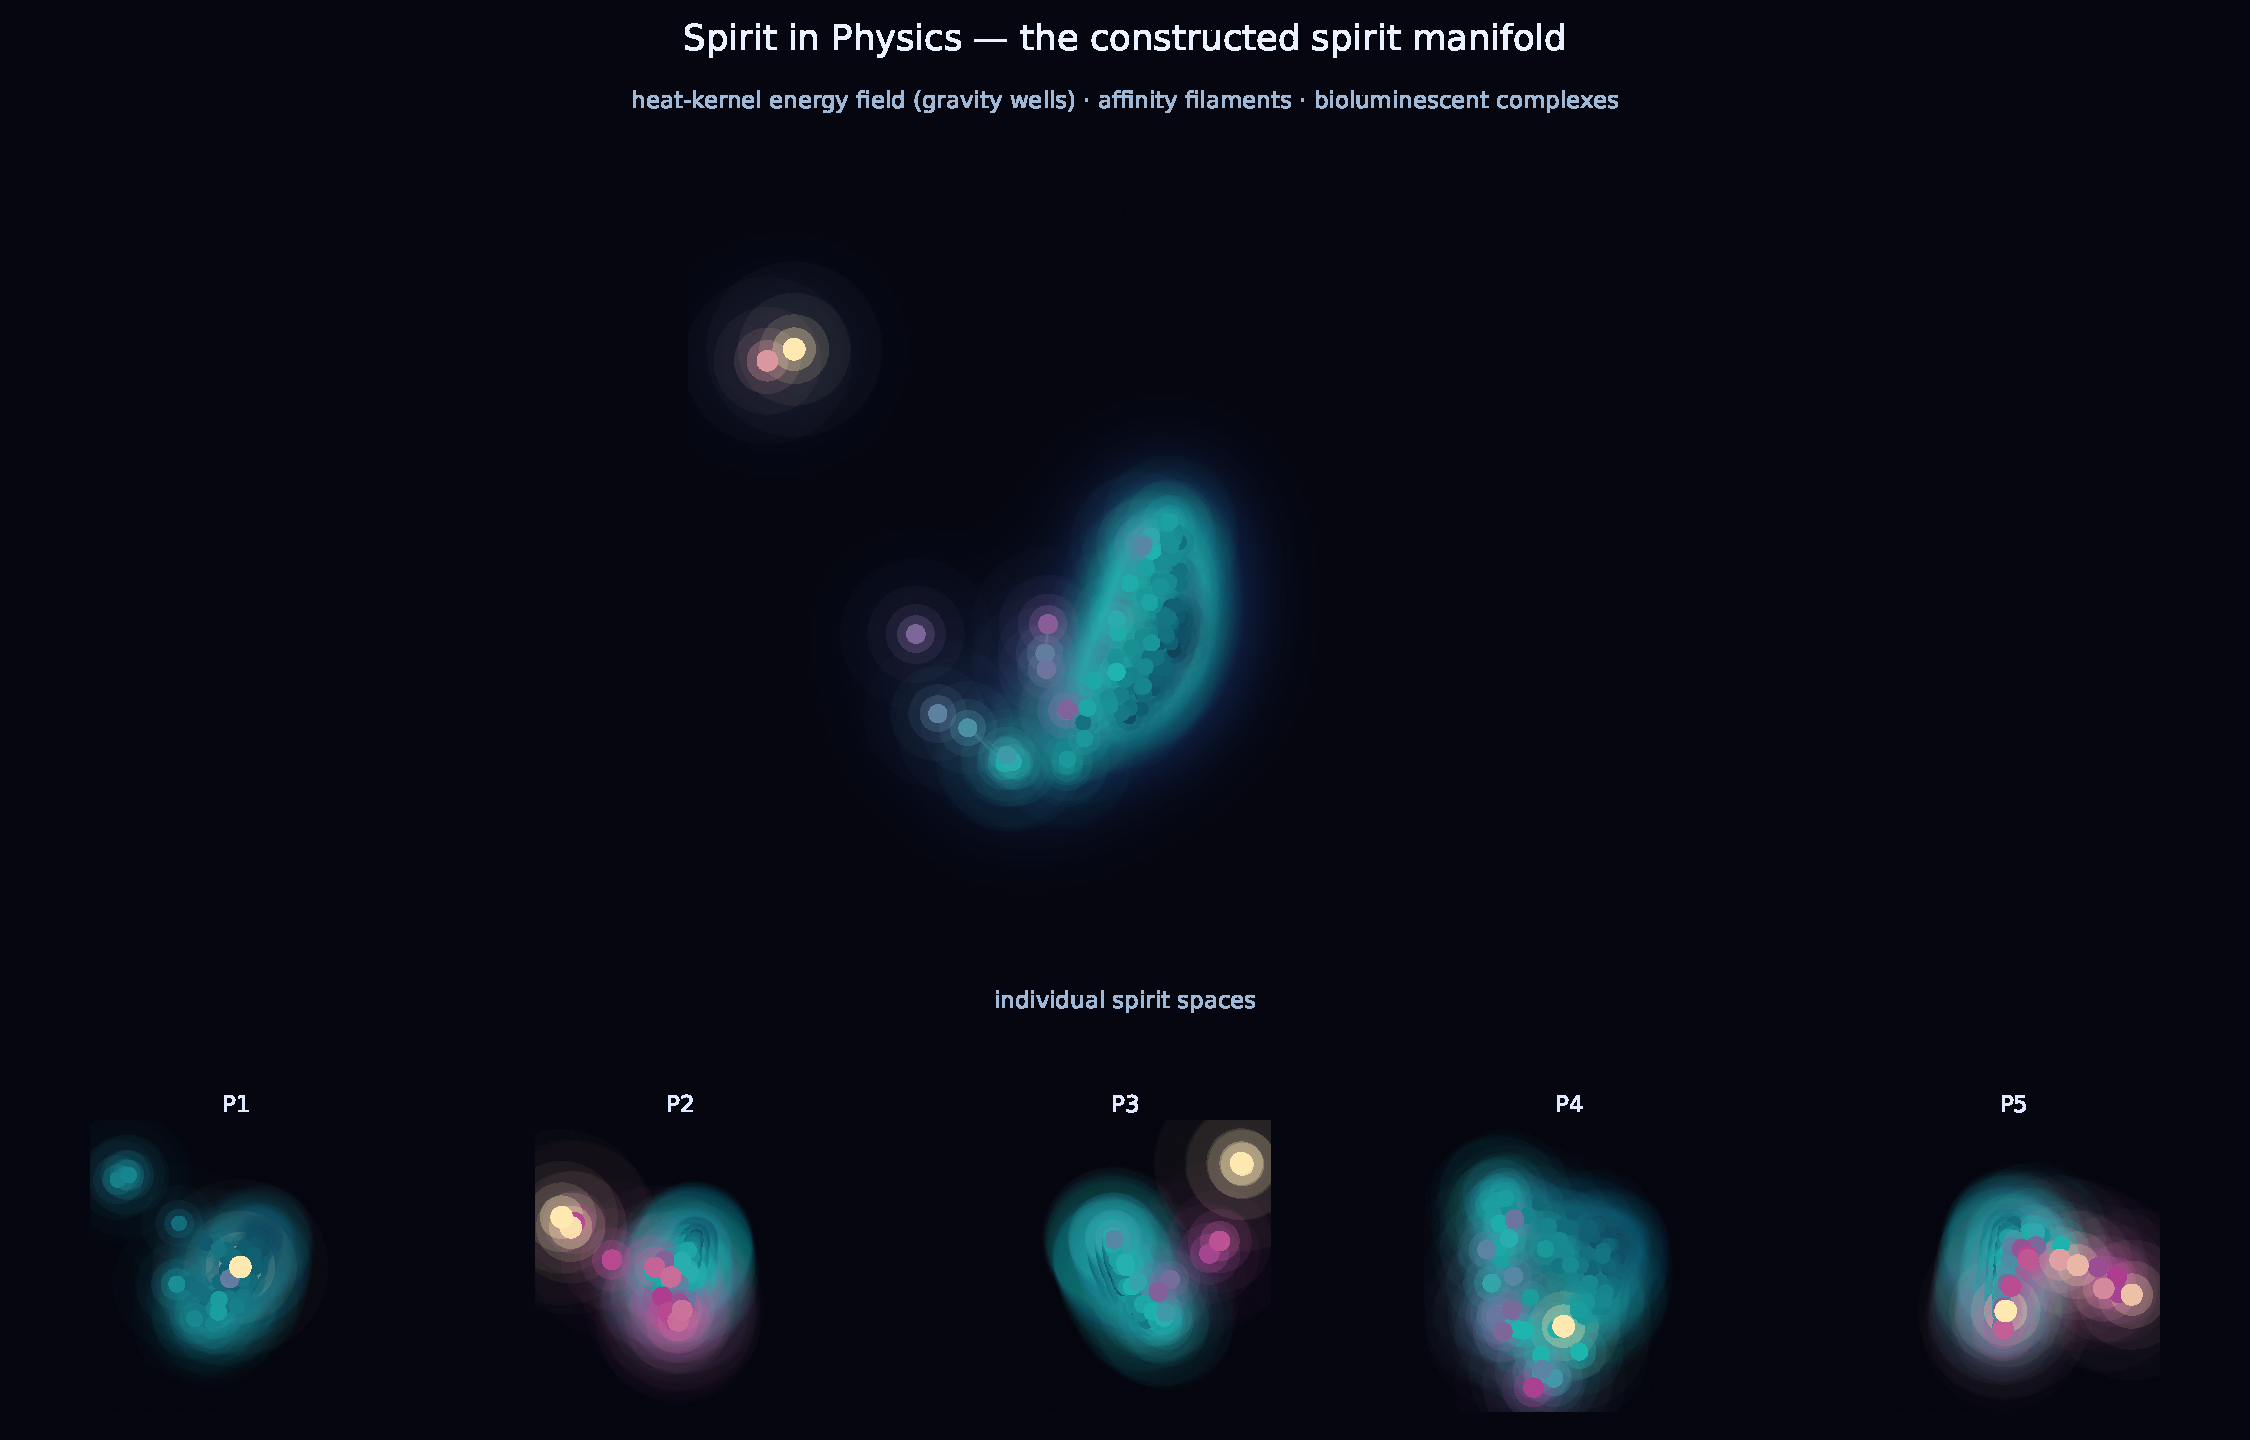
\includegraphics[width=\textwidth]{fig_spirit_awe.pdf}
    \caption{\textbf{The constructed spirit, rendered.} The shared spirit
    manifold (top) and the five individual spirit spaces (bottom), drawn from
    the real spectral embedding, node energy, and affinity kernel. The
    background is the heat-kernel energy field (curved-manifold ``gravity
    wells''); threads are high-affinity edges; bright nodes are high-energy
    complexes. A visualization of the same object the paper constructs---no
    additional data. Generated by \texttt{scripts/render\_spirit\_awe.py}.}
    \label{fig:awe}
\end{figure}

\section{Limitations}
We state the scope plainly. (1) \textbf{Constructive, not confirmatory:} we build and visualize an object under the stated assumption; we do not claim to have tested ``information $=$ physics $=$ spirit'' as a hypothesis. (2) \textbf{Boundary data pending:} the rubber-hand-illusion measurement of the self-boundary---a core element of the method---is not yet collected; the present construction uses word association and physiology only. (3) \textbf{Power:} $N=5$ (of 11). The shared/collective component is at most faint (inter-subject $r=0.07$, $p=0.04$; its variance share sits at the mechanical null), and per-person distinctness is not statistically established (Procrustes ratio $1.08$, $95\%$ CI $[0.46,1.08]$). (4) \textbf{Descriptive geometry:} spectral gap, participation ratio and Tucker ranks are descriptive over $P=5$, not inferential population statistics. (5) \textbf{Thermodynamics:} Landauer is a motivating analogy; no energetic quantity is measured. The powered study will add RHI boundary data, demographics for the cultural/collective analysis, and a pre-registered pipeline.

\paragraph{Data and code availability.} All analysis code is bundled (\texttt{scripts/spirit\_tensor.py}, \texttt{make\_landscape\_figure.py}, \texttt{plot\_spirit\_manifold.py}; the construction also runs as a \texttt{langgraph-clj} StateGraph) and regenerates every figure and number from the raw logs. For byte-stable results the analysis pins Python~3.14 / numpy~2.5 and fixed RNG seeds, so the reported permutation $p$-values ($0.038$, $0.21$) and bootstrap CIs are deterministic; each script regenerates its outputs with a single invocation (e.g.\ \texttt{python scripts/spirit\_tensor.py <stage> state.json}). Raw human-subjects recordings (face/voice, consent) contain personal information and are not publicly released; de-identified derived measures are available from the authors under a data-use agreement, consent permitting.

\section{Conclusion}
We treated ``spirit'' not as a hypothesis to confirm but as an object to construct: under the assumption that the self is information, an individual's spirit \emph{is} the information-geometric space built from their associations and physiology, in which Jungian complexes appear as high-energy regions. A pilot ($N=5$) builds such spaces, locates their complexes from the body alone, and finds the spirit space to be overwhelmingly individual with only a faint, above-chance shared component (candidate collective unconscious, $r=+0.07$, $p=0.04$; its size not estimable at $N=5$) via tensor decomposition. The construction is reproducible and the geometry is real; what remains for the powered, pre-registered study is the physiological boundary (rubber-hand illusion) and the cross-cultural reading of the shared space.

\bibliographystyle{plain}
\bibliography{references}

\end{document}
